\chapter{Methodology} \label{chap:methodology}

In this section, we will formally introduce our experiment. Including the experiment background, the execution plan, the methods and our approaches, as well as our hypothesis for the experiment. Lastly, the expected outcome.

During our literature review section, we explored and discovered a few recent studies on the performance of WebAssembly. Including the comparison between WebAssembly and JavaScript when running in web browsers and the same comparison on native OS environments. The conclusions from those studies are usually favourable towards Webassembly. In addition, with the real-world use case of integrating WebAssembly into web applications, it is not difficult to conclude that WebAssembly performs better than the current implementation across all use cases. However, in this thesis, we argue that this is not true as there need to be more studies on the performance comparison between WebAssembly and the current implementation running on the server-side. Therefore, we will take on this question and fulfil this gap by conducting our own research and undertaking our own experiment.

\bigskip
\section{Introduction and Background}

From the above chapters, we have introduced the concept of WebAssembly and the runtime environments it is currently able to run on, as well as other related topics. Currently, WebAssembly is a trendy topic within the web development industry, but less so outside of it. Therefore, we can undertake a considerable amount of work and research within this area.

For a very long time, companies and organisations deployed and hosted server-side applications on their own servers. That was until the introduction of \textbf{cloud computing}, also known as \textbf{Platform as a service (PaaS)}. Typical cloud computing service providers include \textbf{Amazon Web Services}, which was released all the way back in \textbf{2006} \cite{eva1}, \textbf{Google Cloud Platform} \cite{eva2}, and \textbf{Microsoft Azure} which was released in \textbf{2008} and \textbf{2010}, respectively \cite{eva3}. Cloud computing eliminated the need for individual companies to run, operate and maintain their own servers. Instead, it provides a solution for companies to publish and deploy their applications off-premise. Therefore, it also eliminates the cost of the initial server construction as well as the maintenance of the server.

However, one major issue of cloud computing is \textbf{security}. Anyone can create an application and use the service from PaaS companies to deploy it to the cloud. Therefore, cloud service providers usually have several security features built into their service. One of the most common security features cloud computing companies adopted is containerising clients' applications to individual containers to prevent the application from interacting with the hosting server's operating system. This is a very effective way to improve security measures. However, our literature review discovered that several researchers suggested running applications in containers/virtual machines resulted in worse app performances.

Despite the shortcomings, the container method is adopted by most cloud services, and it is currently the standard, de facto way of publishing and deploying applications to the cloud.

\bigskip
\section{Motivation}

We focused on edge computing a lot in this thesis. We understand that edge computing is getting more popular every day. According to Google searches, we are about \textbf{4} times more interested in edge computing than we were just 5 years ago \cite{exp1}. Large information systems and tech companies have also developed their own edge computing frameworks and products, such as \textbf{Google} with Firebase Cloud Functions \cite{exp2}, \textbf{Cloudflare} with Cloudflare workers \cite{exp3} and \textbf{Vercel} - The creator of Next.js \cite{exp4}, one of the most popular web frameworks, recently entered the edge computing market by introducing edge function for the framework \cite{exp5}.

\newpage
\bigskip
\begin{figure}[hp]
\centering
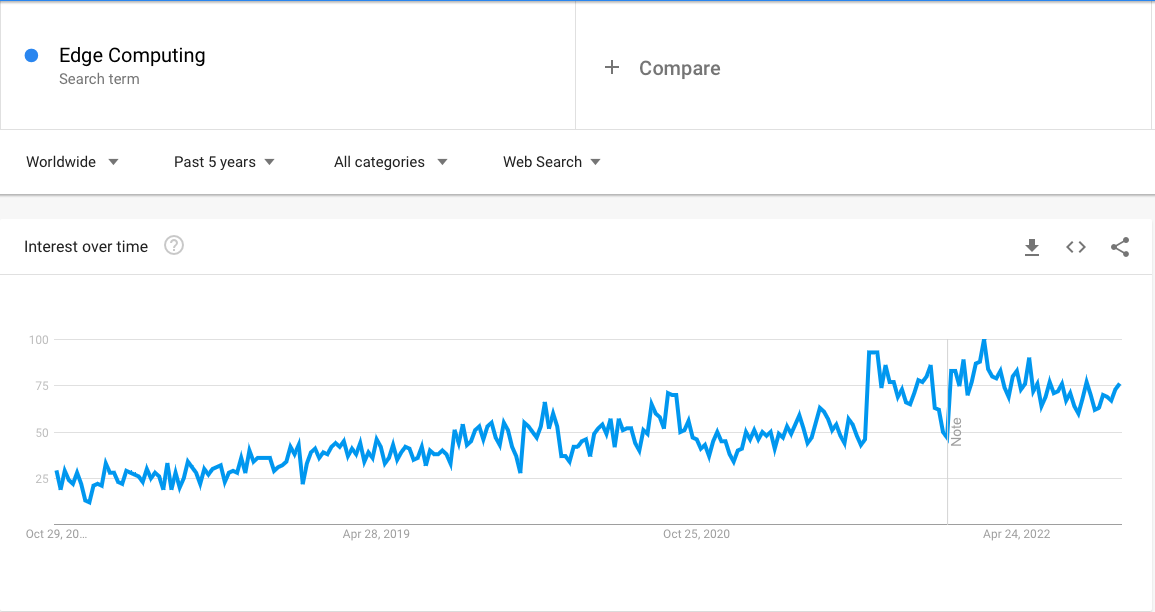
\includegraphics[scale=0.35]{edge-computing-trends}
\caption{\footnotesize{Google trends for edge computing \cite{exp1}}}
\captionsetup{aboveskip=0pt,font=it}
\end{figure}
\bigskip

However, with the current implementation, hosting server-side applications on edge is very inefficient. For example, according to Gadepalli et al. \cite{exp6}, the majority of the current implementation approach is either \textbf{VM-Based (Virtual Machine)} or \textbf{Container-Based}.

For the VM-Based approach, each application is hosted in separate virtual machines within physical hardware. Each virtual machine consists of its own operating system, kernel resource management, library dependencies and language runtimes. These resources will then be utilised to run the application deployed from the client. On the top level, the physical hardware, usually known as a VM manager, manages each of these virtual machines by distributing memory and CPU resources as well as watching the processing thread. This approach is used by a number of well-known cloud service providers. For example, AWS Lambda and Azure Functions \cite{exp7} \cite{exp8}.

The Container-Based implementation uses a more straightforward structure than the VM-Based implementation. With a Container-Based solution, each application will be hosted in containers as per the name suggested. Each container also contains its own library dependencies as well as language runtimes. However, unlike the virtual machine approach, containers have direct access to the hardware's memory and CPU, as well as limited access to specific system APIs. With this method, applications are no longer hosted in virtual machines. Therefore it usually has a faster cold start latency than the VM-Based approach. Popular services such as \textbf{Google Cloud Function} and \textbf{Apache OpenWhisk} use this approach \cite{exp9} \cite{exp10}.

After getting familiarised with the current technology, my natural research instinct kicked in. I kept asking myself if this could be looked into and perhaps researched and experimented with. From all the readings and literature reviews, it is easy to assume that WebAssembly simply has a better performance than the current technology, including when running on the edge. However, we have yet to find the answer, as this is only an assumption. Therefore, we are interested in comparing the two's performances, and we would like to conduct experiments in the environments and scenarios described above.

\begin{figure}[hp]
\centering
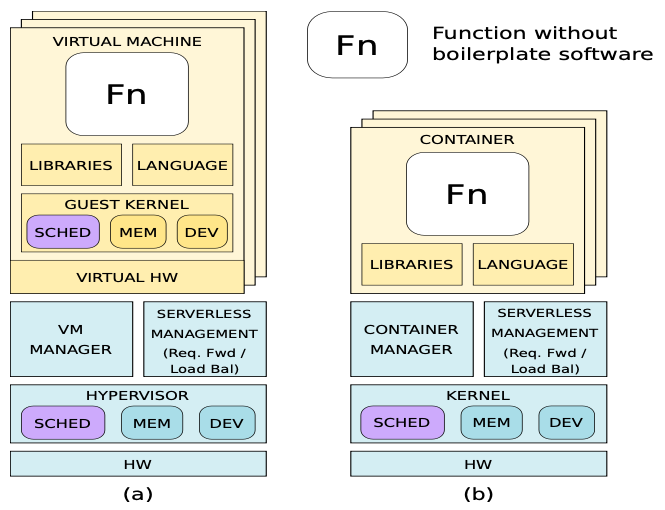
\includegraphics[scale=0.5]{sledge-design-a-b}
\caption{\footnotesize{Visualisation of the current edge computing system design layout, \textbf{a}: VM-Based implementation, \textbf{b}: Container-Based implementation \cite{exp6}}}
\captionsetup{aboveskip=0pt,font=it}
\end{figure}
\bigskip

\bigskip
\section{Our Experiment Goals}

Our experiment involves \textbf{comparing}, \textbf{benchmarking}, and \textbf{analysing} the difference in performance on several aspects between the current way of implementing server-side applications on the cloud, with the newly proposed method of running them with the help of WebAssembly on edge. At the end, we will provide a set of benchmarks that includes the analysed data of the experiment we conducted to contribute to the design and implementation of future commercial WebAssembly frameworks.

Furthermore, we will be listing out and discussing the issues we encountered during our experiment and providing solutions to them to help further research avoid them and improve their research productivity and output.

\bigskip
\section{Improvements and Contribution}

As mentioned above, the current way of developing and deploying server-side applications is neither the most efficient nor cheapest. Applications wrapped in containers while being deployed to a remote server, sometimes on the opposite side of the world, add a considerable amount of \textbf{Round-trip time (RTT)} delay as well as computing overhead. In contrast, the new way of implementation has shown its potential to increase performance by having less overhead and decreasing RTT delay by being distributed on the edge network to be closer to users' physical locations.

We have seen studies showing that when running inside web browsers, WebAssembly outperforms JavaScript on a number of operations and scenarios. This is also reflected by the increasing industry adoption of the technology, with big-name companies such as \textbf{Google} and \textbf{Adobe} migrating major projects from JavaScript to WebAssembly. But, there are very few examples for WebAssembly frameworks being considered and used outside of web browsers, and they have yet to gain too much attention within the industry.

However, this has been changing recently. Multiple studies from the last two years have proposed the idea of running WebAssembly microservices on the server-side and the benefit of doing so. They also developed their own WebAssembly microservice frameworks. In our experiment, we will pick a WebAssembly framework from those implementations and compare that with one of the most popular server-side web frameworks - Python Flask \cite{eva4}.

\newpage
\bigskip
\begin{figure}[hp]
\centering
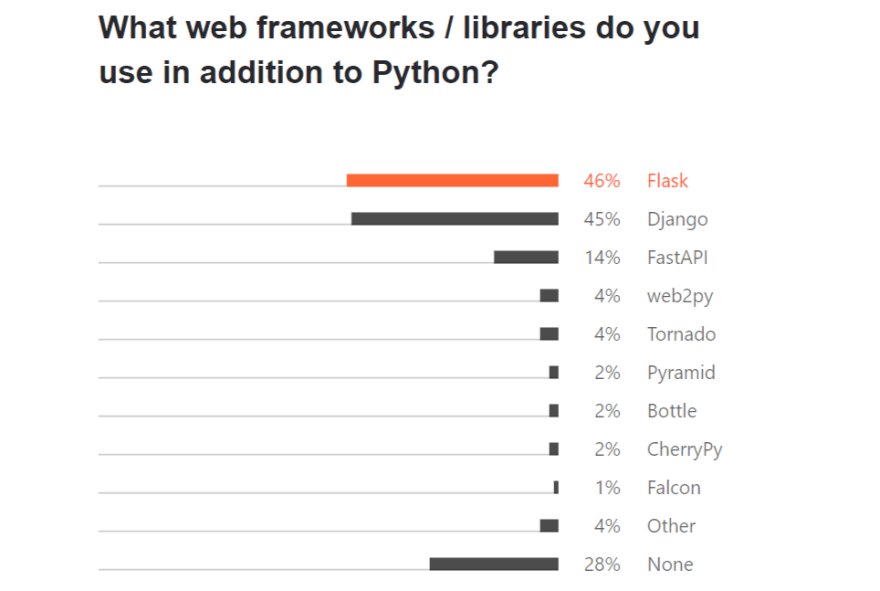
\includegraphics[scale=0.4]{hg2dcbj3lvu2jbjjtdd4}
\caption{\footnotesize{Popularity of major Python web frameworks \cite{eva4}}}
\captionsetup{aboveskip=0pt,font=it}
\end{figure}
\bigskip

\bigskip
\begin{figure}[hp]
\centering
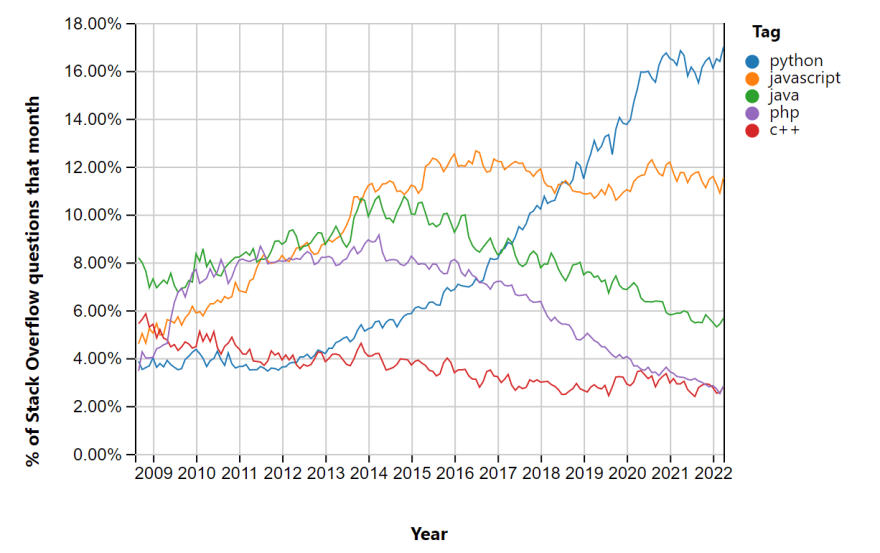
\includegraphics[scale=0.4]{s4fwpypy7bkvtt9kcgr1}
\caption{\footnotesize{Popularity of major programming languages \cite{eva4}}}
\captionsetup{aboveskip=0pt,font=it}
\end{figure}
\bigskip

\bigskip
\section{Hypothesis and Excepted Results}

Since we are undertaking the experiment to either solidify or disprove our expected outcome, we have come up with our own hypothesis for the investigation. From the research and literature review we have undertaken, we understand that WebAssembly has a better performance than JavaScript in web browsers, as well as a faster "code-start" time and lower overhead when running on the server-side. Furthermore, it has a solid technical community to issue updates and patches regularly, as well as work on runtime efficiency and overhead reduction. This resulted in the technology getting more widely adopted as time moved on. Therefore, we consider WebAssembly to be a serious contender in the future of commercial server-side development. And we expect to see a better performance towards the WebAssembly framework in our experiment. We will present our hypothesis in greater detail in the upcoming experiments section.